% ファイル先頭から\begin{document}までの内容(プレアンブル)については,
% 基本的に { } の中を書き換えるだけでよい.
\documentclass[autodetect-engine,dvi=dvipdfmx,ja=standard,
               a4j,11pt]{bxjsarticle}

%%======== プレアンブル ============================================%%
% 用紙設定:指示があれば,適切な余白に設定しなおす
\RequirePackage{geometry}
\geometry{reset,a4paper}
\geometry{hmargin=25truemm,top=25truemm,bottom=25truemm,footskip=10truemm}
%\geometry{showframe} % 本文の"枠"を確認したければ,コメントアウト

% 設定:図の挿入
% http://www.edu.cs.okayama-u.ac.jp/info/tool_guide/tex.html#graphicx
\usepackage{graphicx}

% 設定:ソースコードの挿入
% http://www.edu.cs.okayama-u.ac.jp/info/tool_guide/tex.html#fancyvrb
\usepackage{fancyvrb}
\renewcommand{\theFancyVerbLine}{\texttt{\footnotesize{\arabic{FancyVerbLine}:}}}

%%======== レポートタイトル等 ======================================%%
% ToDo: 提出要領に従って,適切なタイトル・サブタイトルを設定する
\title{システムプログラミング2 \\
       期末レポート}

% ToDo: 自分自身の氏名と学生番号に書き換える
\author{氏名: 重近 大智 (SHIGECHIKA, Daichi) \\
        学生番号: 09501527}

% ToDo: レポート課題等の指示に従って適切に書き換える
\date{出題日: 2020年12月07日 \\
      提出日: \today \\
      締切日: 2020年1月25日 \\}  % 注:最後の\\は不要に見えるが必要.


%%======== 本文 ====================================================%%
\begin{document}
\maketitle
% 目次つきの表紙ページにする場合はコメントを外す
%{\footnotesize \tableofcontents \newpage}

%% 本文は以下に書く.課題に応じて適切な章立てを構成すること.
%% 章=\section,節=\subsection,項=\subsubsection である.

%--------------------------------------------------------------------%
\section{概要} \label{sec:abstract}
本レポートでは,MIPS言語とC言語を用いて,提示された5つの課題に取り組み,その解答を報告する.実行結果はxspim及びgccにより生成された$32$\verb|bit|バイナリによる結果である.

本レポートで報告するシステムプログラミング2の課題は次の5つである.
\begin{enumerate}
\item SPIMが提供するシステムコールをC言語から実行できるようにしたい.A.6節「手続き呼出し規約」に従って,各種手続きをアセンブラで記述せよ\cite{book:assembly}.ファイル名は,\verb|syscalls.s|とすること.また,記述した\verb|syscalls.s|の関数をC言語から呼び出すことで,ハノイの塔(\verb|hanoi.c|とする)を完成させよ.
\item \verb|hanoi.s|を例に\verb|spim-gcc|の引数保存に関するスタックの利用方法について,説明せよ.そのことは,規約上許されるスタックフレームの最小値$24$とどう関係しているか.このスタックフレームの最小値規約を守らないとどのような問題が生じるかについて解説せよ.
\item プログラム\verb|report2-1.c|をコンパイルした結果をもとに,\verb|auto|変数と\verb|static|変数の違い,ポインタと配列の違いについてレポートせよ.
\item \verb|printf|など,一部の関数は,任意の数の引数を取ることができる.これらの関数を可変引数関数と呼ぶ.MIPSのCコンパイラにおいて可変引数関数の実現方法について考察し,解説せよ.
\item \verb|printf|のサブセットを実装し,SPIM上でその動作を確認する応用プログラム(自由なデモプログラム)を作成せよ.フルセットにどれだけ近いか,あるいは,よく使う重要な仕様だけをうまく切り出して,実用的なサブセットを実装しているかについて評価する.ただし,浮動小数は対応しなくてもよい(SPIM自体がうまく対応していない).加えて,この\verb|printf|を利用した応用プログラムの出来も評価の対象とする.
\end{enumerate}


%--------------------------------------------------------------------%
\section{プログラムの説明}\label{sec:capp}
使用したMIPSアセンブリ及びC言語のソースコードは,\ref{sec:makep}章に示す.

\subsection{課題2-1}
まず,\ref{sec:syscall}節に示す\verb|syscalls.s|について説明する.

処理でスタックを確保する必要があるため,\verb|.text|によりテキストセグメントにプログラムを配置する.続いて\verb|.align 2|により次の命令が配置されるメモリ上のアドレスを4バイト境界に整列する.4行目の\verb|_print_int|ラベルから始まる一連の処理は,C言語のソースコードから\verb|print_int()|で呼び出せる処理に相当する.まず\verb|subu|命令でスタックを24バイト確保し,\verb|sw|命令で\verb|$ra|レジスタの値を\verb|$sp + 20|のメモリ上のアドレスに退避する.\verb|li|命令で\verb|$v0|レジスタに1を代入し,システム・コール・コード1である\verb|print_int|を指定する.\verb|syscall|により,システム・コールを行う.その後,\verb|lw|命令で\verb|$ra|レジスタの値をスタックから復元し,\verb|addu|命令でスタックを開放する,\verb|j $ra|により呼び出し元に処理を戻す.

他の\verb|print_string|,\verb|read_int|,\verb|read_string|においては,システム・コール・コードがそれぞれ$4$,$5$,$8$となっていること以外は共通の処理を行っているため,ここでは触れない.なお,\verb|print_int|は実行時の引数に\verb|int|,\verb|print_string|は\verb|char *|,\verb|read_string|は\verb|char *|,\verb|int|の値をそれぞれ渡す必要がある.



\subsection{課題2-5}
続いて,\ref{sec:p2-5}節に示すデモプログラムについて説明する.
まずプログラムの動作を支える\verb|void myprintf(char|

\noindent\verb| *fmt, ...)|関数,\verb|void myscanf(char *fmt, ...)|関数とこれらの関数の動作を支える関数について説明する.

\verb|void print_char(char c)|関数は,1文字を表示する関数で,MIPS言語のシステム・コールでは\verb|print_string(char *)|の形を利用するため,任意の1文字と終端文字をつなぎ合わせた長さ2の配列を作り,その先頭アドレスを\verb|print_string(char *)|に渡す処理を行う.

\verb|void print_big_str(char *s)|関数は,文字列に小文字の英字が含まれる場合,それをすべて大文字にして出力する関数である.引数は\verb|char *|型であり,これにオフセットを加えながら,バッファに1文字分の情報を読み出す.その後ASCIIコードが$97$以上$122$以下の場合は,この値を$-32$して,\verb|print_char(char c)|関数を呼び出す.\verb|void print_small_str(char *s)|関数は,文字列に大文字の英字が含まれる場合,それをすべて小文字にして出力する関数である.ASCIIコードが$65$以上$90$以下の場合は,この値を$+32$して,\verb|print_char(char c)|関数を呼び出す.いずれの関数も戻り値はない.

\verb|char read_char(void)|関数は,1文字入力を受ける関数である.オーバーフロー防止の為,$1024$文字分のバッファを設ける.\verb|read_string(char *, int)|によりシステム・コールを実行する.その後,\verb|c|に\verb|buf[0]|の値を代入し,戻り値とする.

\verb|void myprintf(char *fmt, ...)|関数は,正規の\verb|printf()|の呼び出し時に指定するサブセットに対応する分岐の処理を行う.\verb|char *|型の変数\verb|fmt|で第一引数に対応する文字列の情報を読み取り,その情報の\verb|%|
をもとに変数\verb|i|,\verb|c|,\verb|s|に対応する第二引数以降の情報を代入し,\verb|print_int(int)|,\verb|print_string(char *)|関数などを呼び出す.\verb|%|
とその1文字後のサブセットを指定する英字1文字以外は,\verb|else|文後の\verb|print_char(char c)|関数により,そのまま1文字として出力される.\verb|int|型の変数\verb|argc|が引数の数をカウントし,第一引数が格納されているメモリのアドレスである\verb|&fmt|に,\verb|sizeof(void)|すなわち$4$バイト $*$ \verb|argc|を加えることにより,第二引数以降が格納されているメモリのアドレスを知ることができる.
なお,\verb|myprintf()|関数で使用可能なサブセットは表\ref{tab:printsubsets}に示す.

\verb|void myscanf(char *fmt, ...)|関数は,正規の\verb|scanf()|の呼び出し時に指定するサブセットに対応する分岐の処理を行う.\verb|char *|型の変数\verb|fmt|で第二引数に対応する変数の型の情報を読み取り,その情報をもとにポインタ変数\verb|*i|,\verb|*c|,\verb|*s|に対応する第二引数の情報を代入し,\verb|read_int(int)|,\verb|read_string(char *)|関数などを呼び出す.第一引数が格納されているメモリのアドレスである\verb|&fmt|に,\verb|sizeof(void)|すなわち$4$バイトを加えることにより,第二引数が格納されているメモリのアドレスを知ることができる.
なお,\verb|myscanf()|関数で使用可能なサブセットは表\ref{tab:scansubsets}に示す.また,この\verb|myscanf()|関数は可変引数関数ではなく,第二引数までの制限がある.

デモ内容は,\verb|int|値のみ対応した簡易的な電卓プログラムとなっている.電卓機能はすべて\verb|int main(void)|関数に記述されている.使用可能なコマンドは表\ref{tab:commands}に示す.

\begin{table}[b]
\centering
	\caption{\texttt{myprintf()}関数のサブセット}
	\label{tab:printsubsets}
    	\begin{tabular}{|l|l|}
	\hline
サブセット指定&概要\\
	\hline
\verb|%d|&\verb|int|値出力\\
	\hline
\verb|%c|&1文字出力\\
	\hline
\verb|%s|&文字列出力\\
	\hline
\verb|%B|&文字列中の英小文字は大文字にして出力\\
	\hline
\verb|%b|&文字列中の英大文字は小文字にして出力\\
	\hline

	\end{tabular}
\end{table}

\begin{table}[h]
\centering
	\caption{\texttt{myscanf()}関数のサブセット}
	\label{tab:scansubsets}
    	\begin{tabular}{|l|l|}
	\hline
サブセット指定&概要\\
	\hline
\verb|%d|&\verb|int|値入力\\
	\hline
\verb|%c|&1文字入力\\
	\hline
\verb|%s|&文字列入力\\
	\hline

	\end{tabular}
\end{table}

\begin{table}[b]
\centering
	\caption{電卓で使用可能なコマンド}
	\label{tab:commands}
    	\begin{tabular}{|l|l|}
	\hline
コマンド名&概要\\
	\hline
\verb|+|&加算\\
	\hline
\verb|-|&減算\\
	\hline
\verb|*|&乗算\\
	\hline
\verb|/|&除算\\
	\hline
\verb|0|&計算結果を0に初期化する\\
	\hline
\verb|c|&現在の計算結果を表示する\\
	\hline
\verb|h|&1回前に行った演算を呼び出す\\
	\hline
\verb|q|&正常終了する\\
	\hline

	\end{tabular}
\end{table}


%--------------------------------------------------------------------%
\section{プログラムの使用法と実行結果}\label{sec:howresult}

プログラムは,CentOS 7.6.1810 (Core) のxspimとターミナルで動作を確認している.まず,ターミナルに\verb|xspim &|と打ち込んで,xspimを実行する.
実行後にloadの機能を使い,拡張子が\verb|.s|のアセンブリファイルを読み込む.runの機能で読み込んだプログラムを走らせる.プログラムを走らせた後,もう一度プログラムを走らせる場合には\verb|clear|でメモリとレジスタの値を初期化した後,再度ロードする必要がある.\verb|syscalls.s|(\ref{sec:syscall}節)を用いるプログラムの場合は,最後にこれを読み込ませる.なお,課題2-5のデモプログラムは32bitバイナリを実行し,その実行結果を載せている.

\subsection{課題2-1}
実行結果は次のとおりである.初めに円盤の枚数を尋ねられるので,円盤の枚数を指定する.

\begin{Verbatim}
Enter number of disks> 4
Move disk 1 from peg 1 to peg 3.
Move disk 2 from peg 1 to peg 2.
Move disk 1 from peg 3 to peg 2.
Move disk 3 from peg 1 to peg 3.
Move disk 1 from peg 2 to peg 1.
Move disk 2 from peg 2 to peg 3.
Move disk 1 from peg 1 to peg 3.
Move disk 4 from peg 1 to peg 2.
Move disk 1 from peg 3 to peg 2.
Move disk 2 from peg 3 to peg 1.
Move disk 1 from peg 2 to peg 1.
Move disk 3 from peg 3 to peg 2.
Move disk 1 from peg 1 to peg 3.
Move disk 2 from peg 1 to peg 2.
Move disk 1 from peg 3 to peg 2.
\end{Verbatim}

よって,\verb|hanoi.c|(\ref{sec:hanoi.c}節)をアセンブリした\verb|hanoi.s|(\ref{sec:hanoi.s}節)が正しく動作していることが確認できた.

\subsection{課題2-5}
以下の実行例は,プログラム実行中の動作例を模擬するため,
任意のtxtファイルを標準入力のリダイレクションにより与えることで,実行する例を示している.
通常の利用においては,キーボードから文字列を入力してもよい.

{\fontsize{10pt}{11pt} \selectfont
 \begin{verbatim}
   $ ./a.out < test.txt
 \end{verbatim}
}

以上のようにして,ファイルを標準入力のリダイレクションで与え,32bitバイナリを実行する.
\verb|test.txt|の中身は次のとおりである.
\begin{Verbatim}[fontsize=\small, baselinestretch=0.8]
     1	+
     2	4
     3	0
     4	y
     5	-
     6	2
     7	*
     8	6
     9	/
    10	3
    11	+
    12	4
    13	c
    14	h
    15	y
    16	q
\end{Verbatim}

これをリダイレクションで与えて得られる出力は次のとおりである.

\begin{Verbatim}[fontsize=\small, baselinestretch=0.8]
Starting calculator...
Please select the calc mode. ("+" or "-" or "*" or "/" or "0" or "c" or "h" or "q")
Mode? : Please input the number.(int type ONLY)
Number? : Result : 4

Please select the calc mode. ("+" or "-" or "*" or "/" or "0" or "c" or "h" or "q")
Mode? : Do you want to reset calculation result? (y or N)
Reset calculation result.

Please select the calc mode. ("+" or "-" or "*" or "/" or "0" or "c" or "h" or "q")
Mode? : Please input the number.(int type ONLY)
Number? : Result : -2

Please select the calc mode. ("+" or "-" or "*" or "/" or "0" or "c" or "h" or "q")
Mode? : Please input the number.(int type ONLY)
Number? : Result : -12

Please select the calc mode. ("+" or "-" or "*" or "/" or "0" or "c" or "h" or "q")
Mode? : Please input the number.(int type ONLY)
Number? : Result : -4

Please select the calc mode. ("+" or "-" or "*" or "/" or "0" or "c" or "h" or "q")
Mode? : Please input the number.(int type ONLY)
Number? : Result : 0

Please select the calc mode. ("+" or "-" or "*" or "/" or "0" or "c" or "h" or "q")
Mode? : Result : 0

Please select the calc mode. ("+" or "-" or "*" or "/" or "0" or "c" or "h" or "q")
Mode? : Do you want to calc +4 again? (y or N)
Calculated +4 again.
Result : 4

Please select the calc mode. ("+" or "-" or "*" or "/" or "0" or "c" or "h" or "q")
Mode? : FINAL RESULT : 4
Quit.
\end{Verbatim}

電卓のすべての機能が正しく動作していることが確認できた.なお,xspimにおいても正常に実行可能であることを確認している.

%--------------------------------------------------------------------%
\section{考察} \label{sec:review}

\subsection{課題2-2} \label{sec:stack}
spim-gccを用いてコンパイルを行った場合の\verb|hanoi.s|(\ref{sec:hanoi.s}節)のスタックの確保の一連の処理

\begin{Verbatim}[fontsize=\small, baselinestretch=0.8]
subu    $sp,$sp,24
sw      $ra,20($sp)
sw      $fp,16($sp)
move    $fp,$sp
sw      $a0,24($fp)
sw      $a1,28($fp)
sw      $a2,32($fp)
sw      $a3,36($fp)
\end{Verbatim}

を見ると,まず\verb|subu|命令でスタックポインタの値を$24$減少させる.減少させた後,\verb|sw|命令で\verb|$ra|レジスタの値を\verb|20($sp)|,\verb|fp|レジスタの値を16\verb|($sp)|で示されるメモリ上のアドレスに保存する.これは更新前の\verb|$sp|レジスタの値から見ると,それぞれ$-4$,$-8$されたメモリ上のアドレスを指していることが分かる.同様に\verb|$a0|~\verb|$a3|レジスタの例について考えると,更新前の\verb|$sp|レジスタから見た場合,それぞれ$0$,$4$,$8$,$12$されたメモリ上のアドレスを指している.つまり更新前の\verb|$sp|レジスタより大きいメモリ上のアドレスを指しているため,呼出し側のスタック領域に格納されたことになる.

これを整理すると図\ref{tab:stack}のようになり,各関数のスタック領域はその関数が呼び出されたときの\verb|$fp|レジスタ及び\verb|$ra|レジスタの値,そしてその関数が他の関数を呼び出したときの\verb|$a0|~\verb|$a3|レジスタの値で構成される.それぞれが\verb|32bit|の値であるから計$24$バイト必要となる.もし第5引数以上を要する場合は,$4$バイト$*$(追加で必要な引数の個数)分多くスタックを確保すれば新\verb|$sp|基準で格納される.もし,24バイトより少なく確保してしまうと,次のスタックを確保する際に確保済みのスタックの情報が上書きされ,正しくプログラムが動作しない恐れがある.

\begin{figure}[h]
\centering
  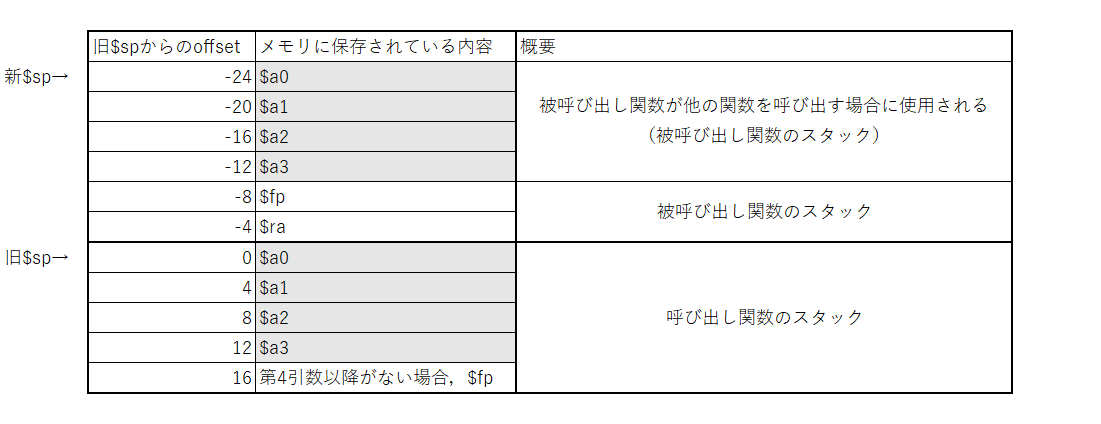
\includegraphics[width=17.0cm]{syspro.png}
	\caption{スタックの状態}
	\label{tab:stack}
\end{figure}

\subsection{課題2-3}
\verb|report2-1.s|(\ref{sec:report2-1.s}節)をもとに\verb|auto|変数と\verb|static|変数について考察すると,64行目からの\verb|main|ラベルの処理
\begin{Verbatim}[fontsize=\small, baselinestretch=0.8]
subu	$sp,$sp,64		# スタックの積立て(64バイト)
sw	$ra,60($sp)		# $sp + 60番地のアドレスに$raの値をバックアップ
sw	$fp,56($sp)		# $sp + 56番地のアドレスに$fpの値をバックアップ
move	$fp,$sp		# $spの値で$fpを上書き
li	$v0,2			# 0x2
sw	$v0,_primes_stat	# _primes_statに対応するラベルのメモリ上のアドレスに$v0の値を保存
li	$v0,3			# 0x3
sw	$v0,16($fp)		# $fp($sp) + 16番地のアドレスに$v0の値をバックアップ
\end{Verbatim}
で64バイトのスタックを確保している.このスタック領域に値を保存しているのが\verb|auto|変数である.値は\verb|$fp|レジスタ,\verb|$sp|レジスタの値にオフセットを合わせて,\verb|lw|命令や\verb|sw|命令でアクセスするため,他の関数を呼び出し,新たにスタックを確保した後にアクセスすることは困難であり,スタックを開放するとアクセスすることは不可能となる.それに対し\verb|static|変数は,データセグメントにあらかじめ長さを決めて確保した領域に値を保存する.変数はラベルを用いてアクセスされるため,他の関数からのアクセスもラベルを使用することで容易にできる.これらの特徴から\verb|auto|変数はスタックを開放し関数が終了してしまうとアクセス不能になり,データセグメントに確保した\verb|static|変数はプログラムを終了するまでアクセス可能であることが分かる.

続いて\verb|report2-1.c|の次の部分で,ポインタと配列について考える.
\begin{Verbatim}[fontsize=\small, baselinestretch=0.8]
char * string_ptr   = "ABCDEFG";
char   string_ary[] = "ABCDEFG";
\end{Verbatim}

\noindent これに対応する\verb|report2-1.s|は,次のとおりである.
\begin{Verbatim}[fontsize=\small, baselinestretch=0.8]
	.rdata			# 読み取り専用データセグメント
	.align	2		# バイト揃え
$LC0:
 	.asciiz	"ABCDEFG"	# 文字列情報
 	.data			# データセグメント
 	.align	2		# バイト揃え
 _string_ptr:			# ポインタ
 	.word	$LC0		# アドレスを参照
 	.align	2		# バイト揃え
 _string_ary:				# 配列
 	.asciiz	"ABCDEFG"	# 文字列情報
\end{Verbatim}

MIPSアセンブリにおいて確保されたポインタは,ここでは\verb|_string_ptr|ラベルから始まる部分に格納されており,ここはデータセグメントである.ポインタであるため,直に文字列情報が格納されているわけではなく,ポインタが指すアドレスの変数の値が文字列の実体である.ここでは\verb|$LC0|ラベルに対応する部分が該当する.なお,この\verb|$LC0|ラベルの部分は読み取り専用データセグメントとなっており,例えばC言語で\verb|*ptr = 'a'|と値を上書きできないことが分かる.MIPSアセンブリにおいて確保された配列は,\verb|_string_ary|ラベルの部分であり,ここに文字列情報を格納している.このラベルのアドレスを基準に文字列情報にアクセス可能で,\verb|$LC0|とは異なりデータセグメントであるため,上書きも可能である.


\subsection{課題2-4}
MIPSのCコンパイラによって生成されたアセンブリを実行した結果,$24$バイトのスタックが確保された場合を考えると,図\ref{tab:stack}の状態になっていることが分かる.スタックの確保と値の代入は\ref{sec:stack}節で触れたため,ここでは触れない.新しい関数を呼び出した際に第一引数,すなわち\verb|$a0|レジスタに対応する値が格納されるスタックの場所は,旧\verb|$sp|が指しているメモリ上のアドレスである.この旧\verb|$sp|からのオフセットを$4$ずつ増加させることで,第二引数以降の値に対応するスタックにアクセスできるため,第一引数が格納されているスタックのアドレスが分かれば第二引数以降の情報も読み取ることができるといえる.\ref{sec:stack}節でも触れたが,第5引数以上を要する場合は,$4$バイト$*$(追加で必要な引数の個数)分多くスタックを確保しておかないと,\verb|$fp|レジスタや\verb|$ra|レジスタに対応するスタックの値を壊してしまいかねないので,余裕を持って確保しておくことが望ましいといえる.C言語においては,第一引数自体のアドレスを\verb|&|を使って取り出し,それに先述したオフセットを加えることで第二引数以降を読み出すことが可能となる.逆にすべての引数を可変にしてしまうと,引数がいくつあるか知る方法がなくなるとともに,基準となる第一引数自体のアドレスも読めなくなってしまうため,これは不可能であるといえる.\verb|myprintf()|関数では,第一引数に対応した文字列の\verb|'%'|の数を数えることで,第二引数以降の引数がいくつあるかを知ることが可能になっている.

%--------------------------------------------------------------------%
\section{感想}
課題2-5において,\verb|myscanf()|関数を可変引数関数にしようとしたが,例えば\verb|myscanf("%d,%s",a ,b);|
として,\verb|int|の値と文字列を\verb|','|で区切って同時に入力可能な仕様にする場合,システム・コールは\verb|print_string()|で行い,その文字列を分割するなどの複雑な処理が必要となるため,今回は実装できなかった.デモプログラムの電卓で例えば\verb|+4|と入力して一気に計算処理ができるようになれば,もっと使いやすくなると思うので改善方法を模索してみたいものである.\verb|myscanf()|関数を自作したことにより,何故正規の\verb|scanf()|関数の第二引数以降の\verb|int|の変数,\verb|char|型の変数で\verb|&|をつけているのかを理解でき,興味深かった.

%--------------------------------------------------------------------%
\section{使用したプログラムのソースコード} \label{sec:makep}

使用したプログラムを以下に添付する.
%なお,\ref{sec:abstract}章に示した課題については,
%\ref{xxxx}章で示したようにすべて正常に動作したことを付記しておく.

% Verbatim environment
% プリアンブルで \usepackage{fancyvrb} が必要.
%   - numbers           行番号を表示.left なら左に表示.
%   - xleftmargin       枠の左の余白.行番号表示用に余白を与えたい.
%   - numbersep         行番号と枠の間隙 (gap).デフォルトは 12 pt.
%   - fontsize          フォントサイズ指定
%   - baselinestretch   行間の大きさを比率で指定.デフォルトは 1.0.

\subsection{\texttt{syscalls.s}} \label{sec:syscall}
\begin{Verbatim}[fontsize=\small, baselinestretch=0.8]
     1      .text
     2      .align 2
     3
     4  _print_int:
     5      subu    $sp,    $sp,    24  # スタックの積立
     6      sw      $ra,    20($sp)     # $raレジスタの値をスタックに退避
     7
     8      li      $v0,    1           # syscall用にprint_intを指定
     9      syscall                     # システムコールの実行
    10
    11      lw      $ra,    20($sp)     # $raレジスタの値の復元
    12      addu    $sp,    $sp,    24  # スタックを解放
    13      j       $ra                 # 呼び出し元に戻る
    14
    15  _print_string:
    16      subu    $sp,    $sp,    24  # スタックの積立
    17      sw      $ra,    20($sp)     # $raレジスタの値をスタックに退避
    18
    19      li      $v0,    4           # syscall用にprint_stringを指定
    20      syscall                     # システムコールの実行
    21
    22      lw      $ra,    20($sp)     # $raレジスタの値の復元
    23      addu    $sp,    $sp,    24  # スタックを解放
    24      j       $ra                 # 呼び出し元に戻る
    25
    26  _read_int:
    27      subu    $sp,    $sp,    24  # スタックの積立
    28      sw      $ra,    20($sp)     # $raレジスタの値をスタックに退避
    29
    30      li      $v0,    5           # syscall用にread_intを指定
    31      syscall                     # システムコールの実行
    32
    33      lw      $ra,    20($sp)     # $raレジスタの値の復元
    34      addu    $sp,    $sp,    24  # スタックを解放
    35      j       $ra                 # 呼び出し元に戻る
    36
    37  _read_string:
    38      subu    $sp,    $sp,    24  # スタックの積立
    39      sw      $ra,    20($sp)     # $raレジスタの値をスタックに退避
    40
    41      li      $v0,    8           # syscall用にread_stringを指定
    42      syscall                     # システムコールの実行
    43
    44      lw      $ra,    20($sp)     # $raレジスタの値の復元
    45      addu    $sp,    $sp,    24  # スタックを解放
    46      j       $ra                 # 呼び出し元に戻る
\end{Verbatim}

\subsection{\texttt{hanoi.c}} \label{sec:hanoi.c}
xspimで実行する場合は,1行目の\verb|#include "spim.h"|は不要である.
\begin{Verbatim}[fontsize=\small, baselinestretch=0.8]
     1  // #include "spim.h"
     2
     3  void hanoi(int n, int start, int finish, int extra)
     4  {
     5    if (n != 0){
     6      hanoi(n - 1, start, extra, finish);
     7      print_string("Move disk ");
     8      print_int(n);
     9      print_string(" from peg ");
    10      print_int(start);
    11      print_string(" to peg ");
    12      print_int(finish);
    13      print_string(".\n");
    14      hanoi(n - 1, extra, finish, start);
    15    }
    16  }
    17
    18  main()
    19  {
    20    int n;
    21    print_string("Enter number of disks> ");
    22    n = read_int();
    23    hanoi(n, 1, 2, 3);
    24  }
\end{Verbatim}

\subsection{\texttt{hanoi.s}} \label{sec:hanoi.s}
\verb|spim-gcc|により生成されたアセンブリコードである.
\begin{Verbatim}[fontsize=\small, baselinestretch=0.8]
     1          .file   1 "hanoi.c"
     2
     3   # -G value = 0, Arch = r2000, ISA = 1
     4   # GNU C version 2.96 20000731 (Red Hat Linux 7.3 2.96-113.2)
nux) compiled by GNU C version 2.96 20000731 (Red Hat Linux 7.3 2.96-
     5   # options passed:  -mno-abicalls -mrnames -mmips-as
     6   # -mno-check-zero-division -march=r2000 -O0 -fleading-unders
     7   # -finhibit-size-directive -fverbose-asm
     8   # options enabled:  -fpeephole -ffunction-cse -fkeep-static-
     9   # -fpcc-struct-return -fsched-interblock -fsched-spec -fbran
g
    10   # -fnew-exceptions -fcommon -finhibit-size-directive -fverbo
    11   # -fgnu-linker -fargument-alias -fleading-underscore -fident
no
    12   # -mrnames -mno-check-zero-division -march=r2000
    13
    14
    15          .rdata
    16          .align  2
    17  $LC0:
    18          .asciiz "Move disk "
    19          .align  2
    20  $LC1:
    21          .asciiz " from peg "
    22          .align  2
    23  $LC2:
    24          .asciiz " to peg "
    25          .align  2
    26  $LC3:
    27          .asciiz ".\n"
    28          .text
    29          .align  2
    30  _hanoi:
    31          subu    $sp,$sp,24
    32          sw      $ra,20($sp)
    33          sw      $fp,16($sp)
    34          move    $fp,$sp
    35          sw      $a0,24($fp)
    36          sw      $a1,28($fp)
    37          sw      $a2,32($fp)
    38          sw      $a3,36($fp)
    39          lw      $v0,24($fp)
    40          beq     $v0,$zero,$L3
    41          lw      $v0,24($fp)
    42          addu    $v0,$v0,-1
    43          move    $a0,$v0
    44          lw      $a1,28($fp)
    45          lw      $a2,36($fp)
    46          lw      $a3,32($fp)
    47          jal     _hanoi
    48          la      $a0,$LC0
    49          jal     _print_string
    50          lw      $a0,24($fp)
    51          jal     _print_int
    52          la      $a0,$LC1
    53          jal     _print_string
    54          lw      $a0,28($fp)
    55          jal     _print_int
    56          la      $a0,$LC2
    57          jal     _print_string
    58          lw      $a0,32($fp)
    59          jal     _print_int
    60          la      $a0,$LC3
    61          jal     _print_string
    62          lw      $v0,24($fp)
    63          addu    $v0,$v0,-1
    64          move    $a0,$v0
    65          lw      $a1,36($fp)
    66          lw      $a2,32($fp)
    67          lw      $a3,28($fp)
    68          jal     _hanoi
    69  $L3:
    70          move    $sp,$fp
    71          lw      $ra,20($sp)
    72          lw      $fp,16($sp)
    73          addu    $sp,$sp,24
    74          j       $ra
    75          .rdata
    76          .align  2
    77  $LC4:
    78          .asciiz "Enter number of disks> "
    79          .text
    80          .align  2
    81  main:
    82          subu    $sp,$sp,32
    83          sw      $ra,28($sp)
    84          sw      $fp,24($sp)
    85          move    $fp,$sp
    86          la      $a0,$LC4
    87          jal     _print_string
    88          jal     _read_int
    89          sw      $v0,16($fp)
    90          lw      $a0,16($fp)
    91          li      $a1,1                   # 0x1
    92          li      $a2,2                   # 0x2
    93          li      $a3,3                   # 0x3
    94          jal     _hanoi
    95          move    $sp,$fp
    96          lw      $ra,28($sp)
    97          lw      $fp,24($sp)
    98          addu    $sp,$sp,32
    99          j       $ra
\end{Verbatim}

\subsection{\texttt{report2-1.c}} \label{sec:report2-1.c}
\begin{Verbatim}[fontsize=\small, baselinestretch=0.8]
     1	int primes_stat[10];
     2	
     3	char * string_ptr   = "ABCDEFG";
     4	char   string_ary[] = "ABCDEFG";
     5	
     6	void print_var(char *name, int val)
     7	{
     8	  print_string(name);
     9	  print_string(" = ");
    10	  print_int(val);
    11	  print_string("\n");
    12	}
    13	
    14	main()
    15	{
    16	  int primes_auto[10];
    17	
    18	  primes_stat[0] = 2;
    19	  primes_auto[0] = 3;
    20	
    21	  print_var("primes_stat[0]", primes_stat[0]);
    22	  print_var("primes_auto[0]", primes_auto[0]);
    23	}
\end{Verbatim}

\subsection{\texttt{report2-1.s}} \label{sec:report2-1.s}
\begin{Verbatim}[fontsize=\small, baselinestretch=0.8]
     1		.file	1 "report2-1.c"
     2	
     3	 # -G value = 0, Arch = r2000, ISA = 1
     4	 # GNU C version 2.96 20000731 (Red Hat Linux 7.3 2.96-113.2) (mipsel-li
nux) compiled by GNU C version 2.96 20000731 (Red Hat Linux 7.3 2.96-113.2).
     5	 # options passed:  -mno-abicalls -mrnames -mmips-as
     6	 # -mno-check-zero-division -march=r2000 -O0 -fleading-underscore
     7	 # -finhibit-size-directive -fverbose-asm
     8	 # options enabled:  -fpeephole -ffunction-cse -fkeep-static-consts
     9	 # -fpcc-struct-return -fsched-interblock -fsched-spec -fbranch-count-re
g
    10	 # -fnew-exceptions -fcommon -finhibit-size-directive -fverbose-asm
    11	 # -fgnu-linker -fargument-alias -fleading-underscore -fident -fmath-err
no
    12	 # -mrnames -mno-check-zero-division -march=r2000
    13	
    14	
    15		.rdata			# 読み取り専用データセグメント
    16		.align	2			# バイト揃え
    17	$LC0:
    18		.asciiz	"ABCDEFG"	# 文字列情報
    19		.data				# データセグメント
    20		.align	2			# バイト揃え
    21	_string_ptr:			# ポインタ
    22		.word	$LC0		# アドレスを参照
    23		.align	2			# バイト揃え
    24	_string_ary:			# 配列
    25		.asciiz	"ABCDEFG"	# 文字列情報
    26		.rdata			# 読み取り専用データセグメント
    27		.align	2			# バイト揃え
    28	$LC1:
    29		.asciiz	" = "		# 文字列情報
    30		.align	2			# バイト揃え
    31	$LC2:
    32		.asciiz	"\n"		# 文字列情報
    33		.text				# テキストセグメント
    34		.align	2			# バイト揃え
    35	_print_var:
    36		subu	$sp,$sp,24	# スタックの積立(24バイト)
    37		sw	$ra,20($sp)		# $sp + 20番地のアドレスに
$raの値をバックアップ
    38		sw	$fp,16($sp)		# $sp + 16番地のアドレスに
$fpの値をバックアップ
    39		move	$fp,$sp		# $spの値で$fpを上書き
    40		sw	$a0,24($fp)		# $fp($sp) + 24番地のアドレ
スに$a0の値をバックアップ(境界跨ぎ)
    41		sw	$a1,28($fp)		# $fp($sp) + 28番地のアドレ
スに$a1の値をバックアップ(境界跨ぎ)
    42		lw	$a0,24($fp)		# 元$a0の値のバックアッ
プをスタックからロード(同時にprint_stringの引数に)
    43		jal	_print_string	# print_stringの呼び出し
    44		la	$a0,$LC1		# "="を指すアドレスを$a0
にロード
    45		jal	_print_string	# print_stringの呼び出し
    46		lw	$a0,28($fp)		# 元$a1の値のバックアッ
プをスタックからロード(同時にprint_stringの引数に)
    47		jal	_print_int		# print_intの呼び出し
    48		la	$a0,$LC2	# "\n"を指すアドレスを$a0にロード
    49		jal	_print_string	# print_stringの呼び出し
    50		move	$sp,$fp		# $fpの値で$spを上書き
    51		lw	$ra,20($sp)		# $sp + 20番地のアドレスか
ら$raの値を復元
    52		lw	$fp,16($sp)		# $sp + 16番地のアドレスか
ら$fpの値を復元
    53		addu	$sp,$sp,24	# スタックの解放
    54		j	$ra				# 呼び出し元に戻る
    55		.rdata			# 読み取り専用データセグメント
    56		.align	2			# バイト揃え
    57	$LC3:
    58		.asciiz	"primes_stat[0]"	# 文字列情報
    59		.align	2			# バイト揃え
    60	$LC4:
    61		.asciiz	"primes_auto[0]"	# 文字列情報
    62		.text					# テキストセグメント
    63		.align	2			# バイト揃え
    64	main:
    65		subu	$sp,$sp,64		# スタックの積立て(64バイト)
    66		sw	$ra,60($sp)				# $sp + 60番地
のアドレスに$raの値をバックアップ
    67		sw	$fp,56($sp)				# $sp + 56番地
のアドレスに$fpの値をバックアップ
    68		move	$fp,$sp			# $spの値で$fpを上書き
    69		li	$v0,2					# 0x2
    70		sw	$v0,_primes_stat		# _primes_statに対応す
るラベルのメモリ上のアドレスに$v0の値を保存
    71		li	$v0,3					# 0x3
    72		sw	$v0,16($fp)				# $fp($sp) + 16
番地のアドレスに$v0の値をバックアップ
    73		la	$a0,$LC3				# "primes_stat[0
]"を指すアドレスを$a0にロード
    74		lw	$a1,_primes_stat		# _primes_statに対応す
るラベルのメモリ上のアドレスの値を$a1にロード
    75		jal	_print_var			# print_varの呼び出し
    76		la	$a0,$LC4				# "primes_auto[0
]"を指すアドレスを$a0にロード
    77		lw	$a1,16($fp)				# 元$v0の値の
バックアップをスタックから$a1にロード(同時にprint_stringの引数に)
    78		jal	_print_var			# print_varの呼び出し
    79		move	$sp,$fp			# $fpの値で$spを上書き
    80		lw	$ra,60($sp)				# $sp + 60番地
のアドレスから$raの値を復元
    81		lw	$fp,56($sp)				# $sp + 56番地
のアドレスから$fpの値を復元
    82		addu	$sp,$sp,64			# スタックの解放
    83		j	$ra				# 呼び出し元に戻る
    84	
    85		.comm	_primes_stat,40	# データセグメントに40バイト確保

\end{Verbatim}

\subsection{課題2-5で用いたコード} \label{sec:p2-5}
xspimで実行する場合は,1行目の\verb|#include "spim.h"|は不要である.
\begin{Verbatim}[fontsize=\small, baselinestretch=0.8]
     1	#include "spim.h"
     2	
     3	void print_char(char c)
     4	{
     5	    char s[2]; // バッファ(2文字目は終端文字)
     6	
     7	    s[0] = c;    // 1文字目代入
     8	    s[1] = '\0'; // 終端文字代入
     9	
    10	    print_string(s); // 文字列表示
    11	}
    12	
    13	void print_big_str(char *s)
    14	{
    15	    int i = 0; // オフセット指定用
    16	    char c;    // 1文字バッファ
    17	
    18	    for (i = 0; *(s + i * sizeof(char)) != '\0'; i++)
    19	    {
    20	        c = *(s + i * sizeof(char)); // 次の文字情報をcに代入
    21	        if (c >= 97 && c <= 122)     // 小文字なら大文字へ
    22	            c -= 32;
    23	        print_char(c); // 1文字表示
    24	    }
    25	}
    26	
    27	void print_small_str(char *s)
    28	{
    29	    int i = 0; // オフセット指定用
    30	    char c;    // 1文字バッファ
    31	
    32	    for (i = 0; *(s + i * sizeof(char)) != '\0'; i++)
    33	    {
    34	        c = *(s + i * sizeof(char)); // 次の文字情報をcに代入
    35	        if (c >= 65 && c <= 90)      // 大文字なら小文字へ
    36	            c += 32;
    37	        print_char(c); // 1文字表示
    38	    }
    39	}
    40	
    41	char read_char() // 1文字入力関数
    42	{
    43	    char buf[1025]; // 入力文字数は最大1024文字
    44	    char c;         // 最初の1文字を格納
    45	
    46	    read_string(buf, 1025); // 入力受付
    47	    c = buf[0];             // 最初の1文字をcに代入
    48	    return c;
    49	}
    50	
    51	void myprintf(char *fmt, ...)
    52	{
    53	    int i;        // 引数から受け取ったint値を代入
    54	    int argc = 0; // 何番目の引数か
    55	    char c;       // 引数から受け取ったASCIIコードを代入
    56	    char *s;      // 引数となる文字列の先頭アドレスを格納
    57	
    58	    while (*fmt)
    59	    {
    60	        if (*fmt == '%')
    61	        {
    62	            fmt++;  // 検索対象文字列を1文字右へ
    63	            argc++; // 引数のカウント数を1増やす
    64	            switch (*fmt)
    65	            {
    66	            case 'd': // 数値の表示
    67	                i = *((int *)((char *)&fmt + argc * sizeof(void *)));
    68	                print_int(i); // 数値表示
    69	                break;
    70	            case 's': // 文字列の表示
    71	                s = *((char **)((char *)&fmt + argc * sizeof(void *)));
    72	                print_string(s); // 文字列表示
    73	                break;
    74	            case 'c': // 1文字表示
    75	                c = *((char *)((char *)&fmt + argc * sizeof(void *)));
    76	                print_char(c); // 1文字表示
    77	                break;
    78	            case 'b': // すべて小文字で表示 *sはchar *
    79	                s = *((char **)((char *)&fmt + argc * sizeof(void *)));
    80	                print_small_str(s);
    81	                break;
    82	            case 'B': // すべて大文字で表示 *sはchar *
    83	                s = *((char **)((char *)&fmt + argc * sizeof(void *)));
    84	                print_big_str(s);
    85	                break;
    86	            }
    87	        }
    88	        else
    89	        {
    90	            print_char(*fmt); // 1文字表示
    91	        }
    92	        fmt++; // 検索対象文字列を1文字右へ
    93	    }
    94	}
    95	
    96	void myscanf(char *fmt, ...) //引数は1個まで
    97	{
    98	    int *i;  // 引数となる変数のアドレスを格納
    99	    char *c; // 引数となる変数のアドレスを格納
   100	    char *s; // 引数となる変数のアドレスを格納
   101	
   102	    while (*fmt)
   103	    {
   104	        if (*fmt == '%')
   105	        {
   106	            fmt++; // 検索対象文字列を1文字右へ
   107	            switch (*fmt)
   108	            {
   109	            case 'd':  // 数値の入力
   110	                i = *((int **)((char *)&fmt + sizeof(void *))); // 代
入先情報
   111	                *i = read_int();
   112	                break;
   113	            case 's':  // 文字列の入力
   114	                s = *((char **)((char *)&fmt + sizeof(void *))); // 代
入先情報
   115	                read_string(s, 1025);
   116	                break;
   117	            case 'c':  // 1文字入力
   118	                c = *((char **)((char *)&fmt + sizeof(void *))); // 代
入先情報
   119	                *c = read_char();
   120	                break;
   121	            }
   122	        }
   123	        fmt++; // 検索対象文字列を1文字右へ
   124	    }
   125	}
   126	
   127	int main() // 整数専用の電卓
   128	{
   129	    int out = 0;        // 計算結果
   130	    int in;             // 計算用の入力数値
   131	    char mode = 'f';    // mode選択用
   132	    char flag;          // y or n フラグ用
   133	    int checkflag = -1; // inの入力の是非(-1:初回時のみ)
   134	    char his_operand;   // 履歴を1回分保存
   135	    int his_num = 0;    // 履歴を1回分保存
   136	
   137	    myprintf("Starting %b...\n", "CALCULATOR");
   138	
   139	    while (1)
   140	    {
   141	        myprintf("Please select the calc mode. (\"+\" or \"-\" or \"*\" 
or \"/\" or \"0\" or \"c\" or \"h\" or \"q\")\nMode? : ", out);
   142	        myscanf("%c", &mode); // mode選択
   143	        if (mode == 'q')      // qを選択した場合
   144	            break;            // whileループを抜ける
   145	
   146	        if (mode == '0') // '0'を選択した場合
   147	        {
   148	            myprintf("Do you want to reset calculation result? (y or N)\
n");
   149	            myscanf("%c", &flag); // フラグ選択
   150	            if (flag == 'y')      // yを選択した場合
   151	            {
   152	                myprintf("Reset calculation result.\n\n");
   153	                out = 0; // 計算結果を0にリセット
   154	            }
   155	            else
   156	                myprintf("Operation cancelled.\n\n");
   157	
   158	            continue;
   159	        }
   160	
   161	        if (mode == 'c') // cを選択した場合
   162	        {
   163	            myprintf("Result : %d\n\n", out); // 確認用に結果を出力
   164	            continue;                         // ループ先頭に戻る
   165	        }
   166	
   167	        if (mode == 'h') // hを選択した場合
   168	        {
   169	            if (checkflag == -1)
   170	            {
   171	                myprintf("Cannot use history func before calculating onc
e.\n\n");
   172	                continue;
   173	            }
   174	
   175	            myprintf("Do you want to calc %c%d again? (y or N)\n", his_o
perand, his_num);
   176	            myscanf("%c", &flag); // フラグ選択
   177	            if (flag == 'y')      // yを選択した場合
   178	            {
   179	                myprintf("Calculated %c%d again.\n", his_operand, his_nu
m);
   180	                mode = his_operand;
   181	                in = his_num;
   182	                checkflag = 1; // inに値を代入したため
   183	            }
   184	            else
   185	            {
   186	                myprintf("Operation cancelled.\n\n");
   187	                continue;
   188	            }
   189	        }
   190	
   191	        if (mode != '+' && mode != '-' && mode != '*' && mode != '/') //
 モードを正しく選択しなかった場合
   192	        {
   193	            myprintf("Please select the correct mode.\n\n");
   194	            continue;
   195	        }
   196	
   197	        if (checkflag <= 0)
   198	        {
   199	            myprintf("Please input the number.(int type ONLY)\nNumber? :
 ");
   200	            myscanf("%d", &in); // 整数の入力値受付
   201	        }
   202	
   203	        his_operand = mode; // historyに入力モードを登録
   204	        his_num = in;       // historyに入力数値を登録
   205	
   206	        if (mode == '+') // 加算モード
   207	            out = out + in;
   208	        if (mode == '-') // 減算モード
   209	            out = out - in;
   210	        if (mode == '*') // 乗算モード
   211	            out = out * in;
   212	        if (mode == '/') // 除算モード
   213	            if (in != 0) // 0除算は禁止
   214	                out = out / in;
   215	            else
   216	                myprintf("Cannot divide by zero.\nOperarion denied.\n");
   217	
   218	        myprintf("Result : %d\n\n", out); // 演算後に結果出力
   219	        checkflag = 0;                    // inは未入力
   220	    }
   221	    myprintf("%B : %d", "final result", out); // 最終結果出力
   222	    myprintf("\nQuit.\n");
   223	    return 0;
   224	}
\end{Verbatim}

%--------------------------------------------------------------------%
% 参考文献
%   以下は,書き方の例である.実際に,参考にした書籍等を見て書くこと.
%   本文で引用する際は,\cite{book:algodata}などとすればよい.
\begin{thebibliography}{99}
  \bibitem{book:assembly} David A. Patterson,John L. Hennessy,コンピュータの構成と設計 第5版[下] -ハードウエアとソフトウエア-,日経BP社,2014.
  %\bibitem{book:label2} 著者名,書名,出版社,発行年.
  %\bibitem{www:label3} WWWページタイトル,URL,アクセス日.
\end{thebibliography}

%--------------------------------------------------------------------%
%% 本文はここより上に書く(\begin{document}\UTF{FF5E}\end{document}が本文である)
\end{document}
